\documentclass[11pt,a4paper]{jsarticle}
\usepackage[dvips]{graphicx}
\usepackage{fancyhdr}
\usepackage{here}
\setcounter{page}{0}
%
\begin{document}

\title{制御工学実験II \\ 論理回路}
\author{提出者 \\ 14104064 下松八重 宏太 \\ \\ 共同実験者 \\ 14101028 梶野 翔平 \\ 14104092 中島 美香 \\ 16104311 北山 拓夢 \\ 13104119 廣瀬 直人}
\date{実験日 \\ 2016年6月28日 \\ 提出日 \\ 2016年7月5日 \\ 再提出日 \\ \today}



\maketitle
\thispagestyle{empty}
\newpage


 \section{目的}
この実験ではディジタル計算機の基礎となる論理回路について理解を深めることを目的とする.
 \section{原理}
  \subsection{ブール代数}
  論理回路では変数が1か0の2つの値しかとらないブール対数を使って処理する.ブール代数の主な定理を以下に示す.\\
 1.$A+0 = A$\ \ \ \ 2.$A \cdot 0 = 0$\ \ \ \ 3.$A+1 = 1$\ \ \ \ 4.$A \cdot 1 = A$\ \ \ \ 5.$A+A = A$ \\
 6.$A \cdot A = A$\ \ \ \ 7.$A+ \bar A = 1$\ \ \ \ 8.$A \cdot \bar A = 0$\ \ \ \ 9.$\overline{\overline{A}} = A$\ \ \ \ 10.$A + A \cdot B = A$ \\
 11.$A \cdot (A + B) = A$\ \ \ \ 12.$A + \bar A \cdot B = A + B$\ \ \ \ 13.$(A+B)\cdot(A+C) = A+B\cdot C$\\
 14.{\it commutative law} \\
   $A+B = B+A$,$A\cdot B = B\cdot A$ \\
 15.{\it asociative law} \\
   $A+B+C = (A+B)+C = A+(B+C)$,$A\cdot B\cdot C = (A\cdot B)\cdot C = A\cdot (B\cdot C)$\\
 16.{\it distributive law} \\
   $A+(B \cdot C \cdot D) = (A+B)\cdot(A+C)\cdot(A+D)$,$A\cdot(B+C+D)=A\cdot B+A\cdot C+A\cdot D$\\
 17.{\it De Morgan's law} \\
   $\overline{(A+B+C)} = \bar{A} \cdot \bar{B} \cdot \bar{C}$,$\overline{(A \cdot B \cdot C)}= \bar A + \bar B + \bar C$ \\
 ただし,``$+$''は論理和(OR)を,``$\cdot$''は論理積(AND)を表す.また,$\bar A$は$A$の否定(NOT)を表す.

  \subsection{論理素子}
  論理回路を構成する素子のうち代表的なものを図\ref{fig1}に示す.また,これらの真理値表を\ref{tab1}に示す.しかし,実際の論理回路ではNAND素子のみを用いて他の素子を実現している.各論理素子をNAND素子で表したものを\ref{fig2}に示す.

\newpage
\begin{figure}[hb]
 \begin{center}
  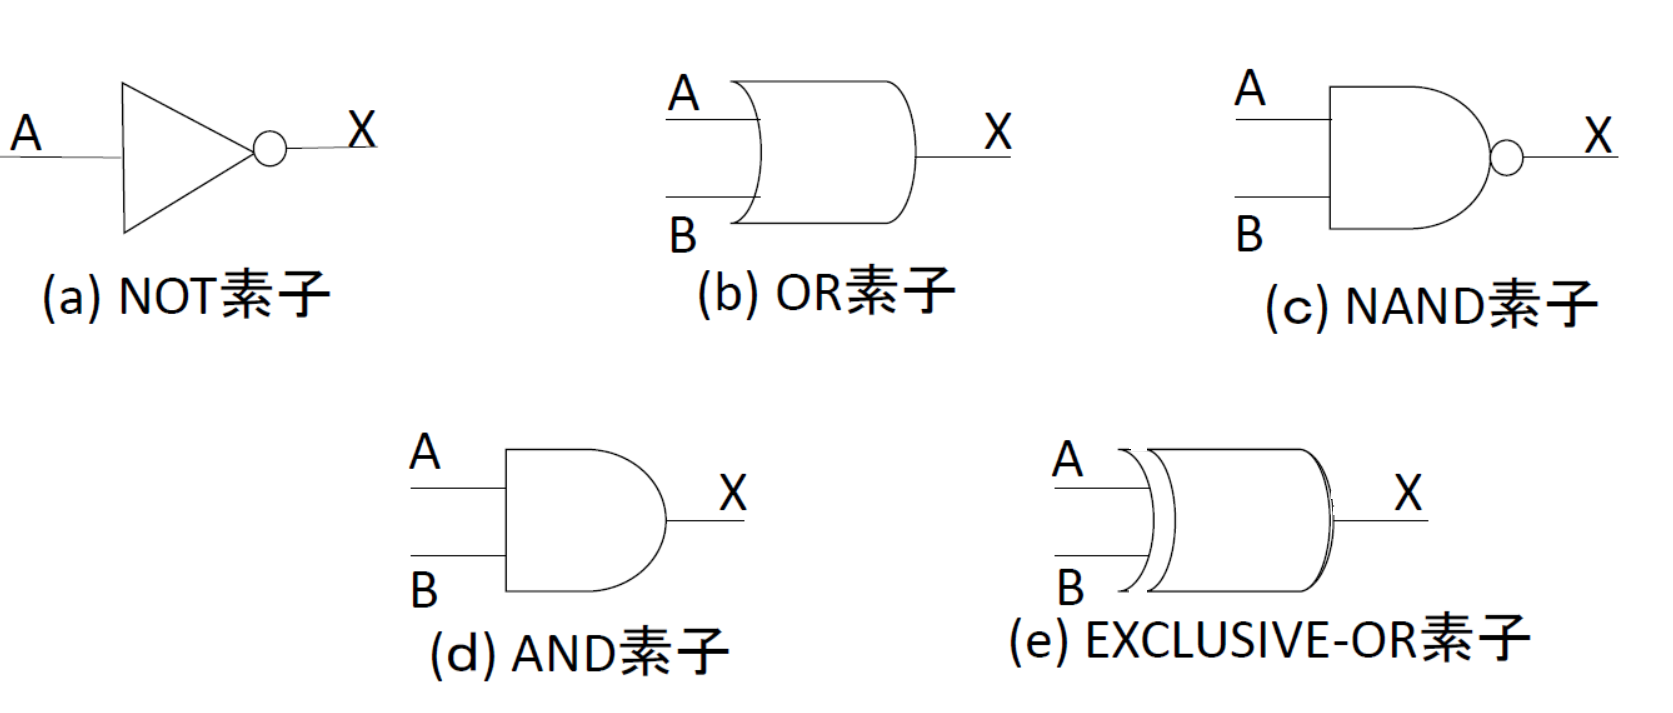
\includegraphics[scale = .3]{./picture/screen.eps}
 \end{center}
 \caption{代表的な論理回路}
\label{fig1}
\end{figure}


\begin{figure}[hb]
 \begin{center}
  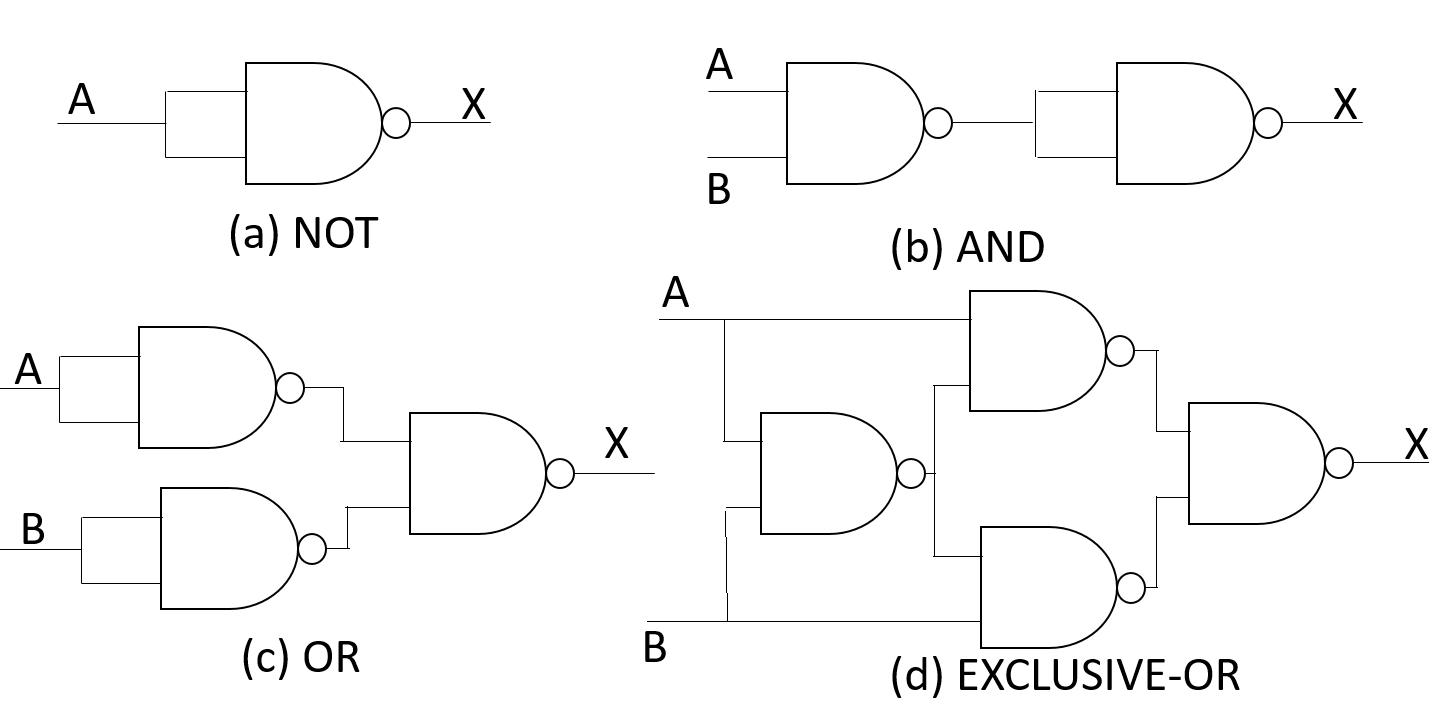
\includegraphics[scale = .3]{./picture/screen2.eps}
 \end{center}
\caption{NAND素子で表した各回路}
\label{fig2}
\end{figure}


\begin{table}[ht]
 \begin{center}
  \caption{真理値表}
  \label{tab1}
  \begin{tabular}{|c|c|c|c|} \hline 
       & A & B & X \\ \hline \hline
   NOT & 0 & - & 1 \\ \cline{2-4}
       & 1 & - & 0 \\ \hline
       & 0 & 0 & 0 \\ \cline{2-4}
   AND & 0 & 1 & 0 \\ \cline{2-4}
       & 1 & 0 & 0 \\ \cline{2-4}
       & 1 & 1 & 1 \\ \hline
       & 0 & 0 & 0 \\ \cline{2-4}
   OR  & 0 & 1 & 1 \\ \cline{2-4}
       & 1 & 0 & 1 \\ \cline{2-4}
       & 1 & 1 & 1 \\ \hline
       & 0 & 0 & 0 \\ \cline{2-4}
EXCLUSIVE-OR & 0 & 1 & 1 \\ \cline{2-4}
       & 1 & 0 & 1 \\ \cline{2-4}
       & 1 & 1 & 0 \\ \hline
       & 0 & 0 & 1 \\ \cline{2-4}
  NAND & 0 & 1 & 1 \\ \cline{2-4}
       & 1 & 0 & 1 \\ \cline{2-4}
       & 1 & 1 & 0 \\ \hline
  \end{tabular}
 \end{center}
\end{table}

\newpage



  \subsection{フリップフロップ}
  フリップフロップは論理回路で用いられる記憶素子であり,RS-FF,JK-FF,T-FF,D-FFなどがある.この実験ではRS-FF回路を使用する.

 \section{実験方法}
 論理回路実験装置を用いて以下の論理回路を実験装置上に実現し,2.について出力を求め真理値表を作製する.
\begin{enumerate}
 \item NOT,AND,OR,EXCLUSIVE-OR素子(表\ref{tab1}となるように確認)
 \item $F = B\bar C(A+\bar D)+ACD+\bar A\bar BCD+\bar A\bar B\bar D$
 \item RS-FF(動作の確認)
\end{enumerate}

\section{結果}
  \subsection{与えられた論理回路について}
  与えられた式をカルノー図を用いて簡略化すると,
  \begin{eqnarray*}
   F = \bar A\bar C\bar D + AB\bar C + ACD + \bar A\bar BC
  \end{eqnarray*}
  となる.真理値表を表\ref{tab2}に示す.また,回路図を図\ref{fig3}に示す.
  
  \begin{table}[h]
   \centering
 \caption{真理値表}
   \label{tab2}
   \begin{tabular}{|c|c|c|c||c|c|c|c||c|} \hline
    $A$ & $B$ & $C$ & $D$ & $\bar A\bar C\bar D$ & $AB\bar C$ & $ACD$ & $\bar A\bar BC$ & $F$\\ \hline
    0& 0& 0& 0&1 &0 &0 &0 & 1\\ \hline
    0& 0& 0& 1& 0& 0& 0&0 & 0\\ \hline
    0& 0& 1& 0& 0& 0& 0& 1& 1\\ \hline
    0& 0& 1& 1& 0& 0& 0& 1& 1\\ \hline
    0& 1& 0& 0& 1& 0& 0& 0& 1\\ \hline
    0& 1& 0& 1& 0& 0& 0& 0& 0\\ \hline
    0& 1& 1& 1& 0& 0& 0& 0& 0\\ \hline
    1& 0& 0& 0& 0& 0& 0& 0& 0\\ \hline
    1& 0& 0& 1& 0& 0& 0& 0& 0\\ \hline
    1& 0& 1& 0& 0& 0& 0& 0& 0\\ \hline
    1& 0& 1& 1& 0& 0& 1& 0& 1\\ \hline
    1& 1& 0& 0& 0& 1& 0& 0& 1\\ \hline
    1& 1& 0& 1& 0& 1& 0& 0& 1\\ \hline
    1& 1& 1& 0& 0& 0& 0& 0& 0\\ \hline
    1& 1& 1& 1& 0& 0& 1& 0& 1\\ \hline
   \end{tabular}
  \end{table}

\begin{figure}[H]
 \begin{center}
  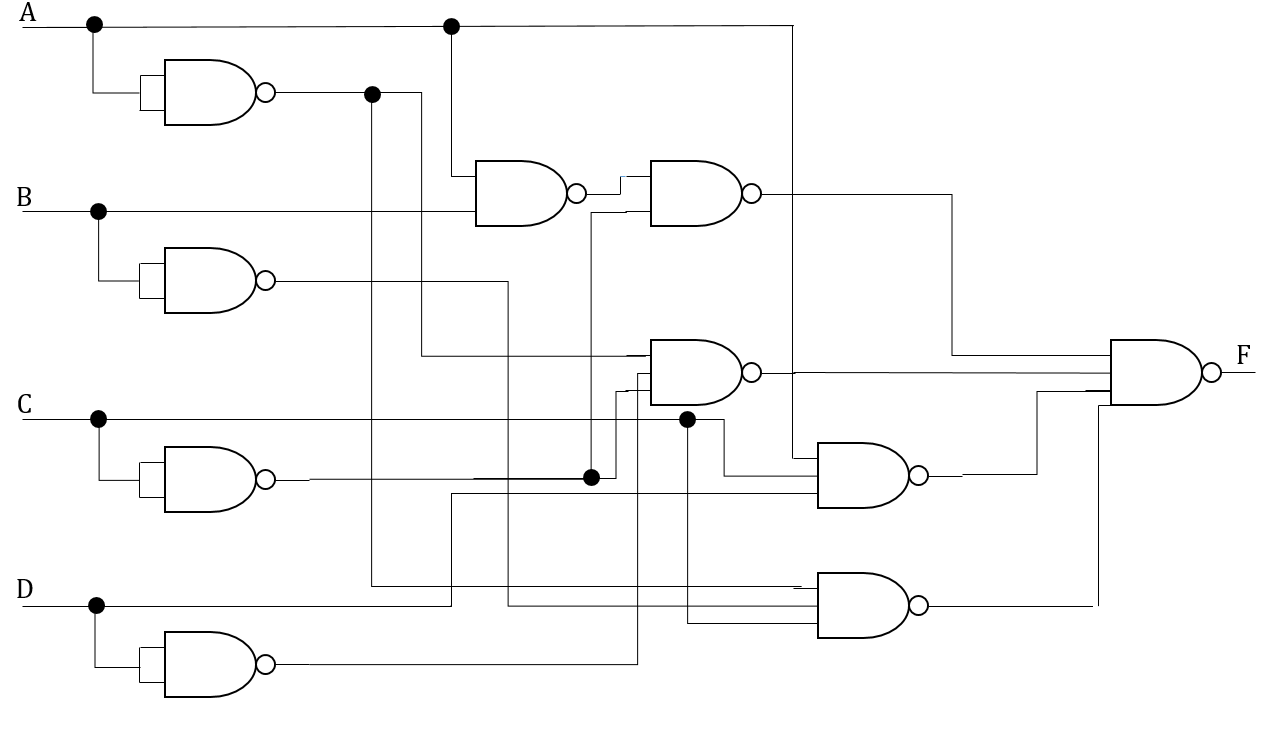
\includegraphics[scale = .5]{./picture/logic.eps}
  \caption{論理回路図}
  \label{fig3}
 \end{center}
\end{figure}


\newpage
\thispagestyle{fancy}
\rhead{再1}
\cfoot{}
\setcounter{section}{1}

\section{原理}
\subsection{RS-FFについて}
RS-FFをNAND素子で表し,その出力を図\ref{fig4}に示す.それぞれの添字$n$は入力が$n$回切り替わった事を示す.\\
 ここで,$n$回目の入力切り替えの結果,RS-FFの出力が$Q_n = 0,\bar{Q_n} = 1$となったとする.$(n+1)$回目の入力切り替えで$S_{n+1} = 1,R_{n+1} = 0$になったとすると,まず$X_1 = 0,X_2 = 1$となる.これより,$N_3$の出力は$X_3 = 1$,すなわち$Q_{n+1} = 1$となる.次に$N_4$には$X_2 = 1,X_3 = 1$が入力されるため$X_4 = 1$となる.同様にして入出力の組み合わせを考え,真理値表を作成すると表\ref{tab2}となる.
また,入力が$R=S=1$のときの出力は$(Q_{n+1},\bar Q_{n+1}) = (1,0)$か,あるいは$(Q_{n+1},\bar Q_{n+1}) = (0,1)$のどちらか予測出来ないため,この入力の組み合わせは禁止である.

\begin{figure}[h]
 \begin{center}
  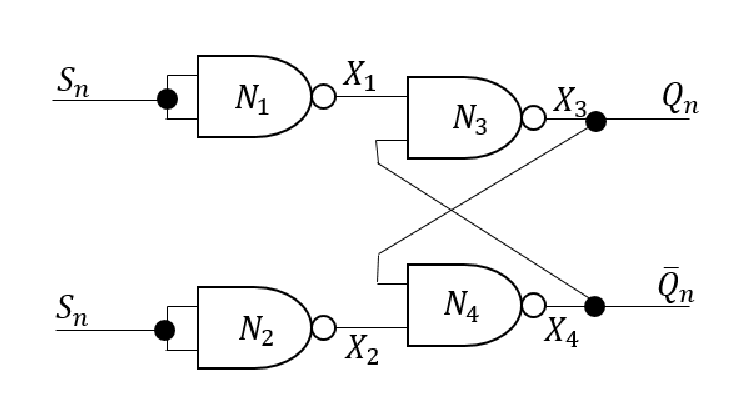
\includegraphics[scale=.7]{./picture/rsff.eps}
  \caption{RS-FF}
\label{fig4}
 \end{center}
\end{figure}

\begin{table}[h]
\centering
 \caption{RS-FFの真理値表}
 \label{tab2}
 \begin{tabular}{|c|c|c|c|} \hline
 \multicolumn{2}{|c|}{入力}& \multicolumn{2}{|c|}{出力} \\ \hline
  $S$ & $R$ & $Q_{n+1}$ & $\overline{Q_{n+1}}$ \\ \hline
    0 &  0  & $Q_n $    & $\overline{Q_n}$     \\ \hline
    0 &  1  &      0    &        1             \\ \hline
    1 &  0  &      1    &        0             \\ \hline
    1 &  1  &     不定  &      不定             \\ \hline
 \end{tabular}
\end{table}

\newpage
\thispagestyle{fancy}
\rhead{再2}
\cfoot{}


\setcounter{section}{4}
\section{課題}
\subsection{カルノー図による論理式の簡略化}
与えられた式をカルノー図を用いて簡略化する.まず,線形性より
\begin{eqnarray*}
F & = & B\bar C(A+\bar D)+ACD+\bar A\bar BCD+\bar A\bar B\bar D \\
  & = & B\bar C A + B\bar C \bar D + ACD + \bar A \bar B CD + \bar A \bar B \bar D \\
\end{eqnarray*}
この式よりカルノー図を作成し,表\ref{tab3}に示す.



\begin{table}[hb]
 \begin{center}
  \begin{tabular}{|c|c|c|c|c|c|} \hline
   &&\multicolumn{2}{|c|}{$\bar C$} & \multicolumn{2}{|c|}{$C$} \\ \cline{3-6} 
   &&$\bar D$ & \multicolumn{2}{|c|}{$D$} & $\bar D$  \\ \hline
   $\bar A$ &$\bar B$& 1 &   & 1 & 1 \\ \cline{2-6}
            &$B$     & 1 &   &   &   \\ \hline
   $A$      &$B$     & 1 & 1 & 1 &   \\ \cline{2-6}
            &$\bar B$&   &   & 1 &   \\ \hline
  \end{tabular}
  \caption{カルノー図}
  \label{tab3}
 \end{center}
\end{table}

この図より,1のマス目を最も大きな$2^n$個の規則的なマス目を囲み,そこに該当する式を表現すると
\begin{eqnarray*}
 F & = & \bar A \bar C \bar D + AB\bar C + ACD + \bar A \bar B C \\
   & = & \overline{\overline{\bar A \bar C \bar D}} + \overline{\overline{AB \bar C}} + \overline{\overline{ACD}} + \overline{\overline{\bar A \bar B C}} \\
   & = & \overline{\overline{\bar A \bar C \bar D} \cdot \overline{AB \bar C} \cdot \overline{ACD} \cdot \overline{\bar A \bar B C}} \\
   & = & \overline{\overline{\overline{AA} \  \overline{CC} \  \overline{DD}} \cdot \overline{AA \overline{CC}} \cdot \overline{ACD} \cdot \overline{\overline{AA} \ \overline{BB} C}}
\end{eqnarray*}
となり,これでこの論理式をNAND素子で表すことができる.論理回路を図\ref{fig4}に示す.


\newpage
\thispagestyle{fancy}
\rhead{再3}
\cfoot{}

\newpage

\subsection{RS-FFについて}
RS-FFにおいて,$R = 1,S = 1$とした時,出力は不定となる.これは厳密に同時に$R = 1,S = 1$とすることは出来ず,必ずどちらかの入力が1となった後にもう一方が1となるためであると考えられる.

  \subsection{論理回路について}
論理回路は論理演算を行う為の電気回路で,基本的にディジタル回路である.論理演算で用いる論理変数は0と1の2つで,電圧をある値で高低の区間に分けたりしてディジタル信号をアナログ電圧で表している.論理回路によって計算機などで様々な状態を表現することが出来る.


  \subsection{QM法による論理式の簡略化}
  QM法(クワイン・マクラスキー法)とはカルノー図による簡略化が複雑になる4変数以上の論理を簡単化する方法として有効な方法である.クワイン部とマクラスキー部によって構成され,クワイン部で主項の導出,マクラスキー部で最小形を導出する.
   \subsubsection{クワイン部による主項の導出}
表\ref{tab2}の真理値表より,結果が1となっている部分をMin\ $i$\ ($i$ = 1,2,3,…)として以下の論理和標準形を求める.
\begin{eqnarray*}
 {\rm Y = Min0 + Min1 + ・・・+Min\ {\it n}} \nonumber
\end{eqnarray*}
 次に,各最小項を含まれる1の数でグループ分けする.結果を表\ref{tab4}に示す.

\begin{table}[b]
 \centering
 \caption{グループ分けの結果}
 \label{tab4}
 \begin{tabular}{|c|c|c|c|c|c|} \hline
  1の個数 &  0  &  1  &  2  &  3  &  4  \\ \hline
          &0000(0) &0001(1) &0011(3) &1011(5) &1111(8) \\ 
  項($i$) &     &0010(2) &1100(6) &1101(7) &     \\ 
          &     &0100(4) &     &     &     \\ \hline 
 \end{tabular}
\end{table}
 隣り合うグループの全ての組み合わせを考え,変数の比較を行う.1変数のみが異なる組み合わせに関して異なっている変数をドント・ケアdに置き換え,2つの項を結合する.結合後の()内に結合前の値を小さい順に記述する.結合結果を表\ref{tab5}に示す.

\thispagestyle{fancy}
\rhead{再2}
\cfoot{}
\begin{table}[H]
 \begin{center}
  \caption{1回目の結合結果}
  \label{tab5}
  \begin{tabular}{|c|c|c|c|c|} \hline
   1の個数 & 0 & 1 & 2 & 3 \\ \hline
           &000d(0,1) &00d1(1,3) &d011(3,5) &11d1(7,8) \\ 
  項($i$)  &          &001d(2,3) &110d(6,7) &          \\ 
           &          &d100(4,6) &          &          \\ \hline
  \end{tabular}
 \end{center}
\end{table}
 これをすべての項が結合できなくなるまで繰り返す.ただしdを持つ項に関しては,同じ位置にdを持つものとのみ結合可能とする.結果を表\ref{tab6}に示す.残った項が主項となる.
 \begin{table}[H]
  \centering
  \caption{最終的な結合結果}
  \label{tab6}
  \begin{tabular}{|c|c|c|c|c|} \hline
   1の個数 & 0 & 1 & 2 & 3 \\ \hline
           &00dd(0,1,2,3) &00d1(1,3) &d011(3,5) &11d1(7,8) \\ 
   項($i$) &              &d100(4,6) &110d(6,7) &          \\  \hline
  \end{tabular} 
 \end{table}

   \subsubsection{マクラスキー部による最小部の導出}
   最小論理和形や最小論理積形を求めるにはクライン部で求めた主項より必須主項を選択する必要がある.マクラスキー部はこれを選択する手法である.\\
    まず主項と対応する最小項の表を作成し,主項がカバーする箇所に印をつける.(表\ref{tab7})

\begin{table}[h]
 \centering
\caption{主項と最小項の対応}
\label{tab7}
 \begin{tabular}{|c|c|c|c|c|c|c|c|c|c|} \hline
  最小項$i$    & 0 & 1 & 2 & 3 & 4 & 5 & 6 & 7 & 8 \\ \hline
  00dd(0,1,2,3)& - & - & - & - &   &   &   &   &   \\ \hline
  00d1(1,3)    &   & - &   & - &   &   &   &   &   \\ \hline
  d100(4,6)    &   &   &   &   & - &   & - &   &   \\ \hline
  d011(3,5)    &   &   &   & - &   & - &   &   &   \\ \hline
  110d(6,7)    &   &   &   &   &   &   & - & - &   \\ \hline
  11d1(7,8)    &   &   &   &   &   &   &   & - & - \\ \hline
\end{tabular}
\end{table}
 最小項の列に注目して,1つのみの主項($i$)でカバーされているものに印をつける.これによって得られた主項でカバー出来る項があれば,全てに印をつける.その後,最小項にカバーされていないものがあれば,それを選び,必須主項に追加する.必須主項となった部分に1を入れて表にしたものを表\ref{tab8}に示す.
 得られた必須主項に対して,1を真,0を偽,dは無視して論理積を求める.これらの論理和が求める最小論理和形となる.つまり,(00dd)は$\bar A \bar B$となる.従って,最小論理和形は以下のとおりである.
\begin{eqnarray*}
 F = \bar A \bar B + B \bar C \bar D + \bar B CD + ACD
\end{eqnarray*}

\thispagestyle{fancy}
\rhead{再4}
\cfoot{}

\newpage
\thispagestyle{fancy}
\rhead{再5}
\cfoot{}


\begin{table}[H]
 \centering
 \caption{必須主項}
 \label{tab8}
 \begin{tabular}{|c|c|c|c|c|c|c|c|c|c|} \hline
  最小項$i$    & 0 & 1 & 2 & 3 & 4 & 5 & 6 & 7 & 8 \\ \hline
  00dd(0,1,2,3)& 1 & 1 & 1 & 1 &   &   &   &   &   \\\hline 
  00d1(1,3)    &   & - &   & - &   &   &   &   &   \\  \hline 
  d100(4,6)    &   &   &   &   & 1 &   & 1 &   &   \\  \hline 
  d011(3,5)    &   &   &   & 1 &   & 1 &   &   &   \\  \hline 
  110d(6,7)    &   &   &   &   &   &   & - & - &   \\  \hline 
  11d1(7,8)    &   &   &   &   &   &   &   & 1 & 1 \\  \hline 
 \end{tabular}
\end{table}


\begin{thebibliography}{9}
 \bibitem[1] 浅川 毅,``論理回路の設計'',コロナ社,2007,pp47-53.
 \bibitem[2] 安藤 繋,``電子回路'',培風館,2006,p79.
\end{thebibliography}

\newpage
\pagestyle{fancy}
\setcounter{page}{1}
\setcounter{section}{3}
\renewcommand{\thepage}{$再々$\,\arabic{page}}
\renewcommand{\headrulewidth}{0.0pt}
\rhead{\thepage}
\lhead{}
\cfoot{}


\section{結果}
\subsection{基本的な論理回路素子の確認}
NAND素子を用いてNOT,AND,OR,EXCLUSIVE-OR素子を図2の回路図の通りに作製し,その入出力関係が表1のようになることを確認した.

\setcounter{subsection}{2}

\subsection{RS-FF}
実験装置上でRS-FFを作製しその入出力関係が表3のようになる事を確認した.


\begin{thebibliography}{9}
 \bibitem[1]  浅川 毅,``論理回路の設計'',コロナ社,pp.47-53,2007.
 \bibitem[2]  安藤 繋,``電子回路'',培風館,pp.79,2006.
\end{thebibliography}


\end{document}





